\section{Sicherheit}
\subsection{Allgemeine Sicherheitshinweise}
Der entwickelte Probenverdünner dient ausschließlich dem zuvor beschriebenen Zweck (\autoref{ZweckDesGeraets}) der Verdünnung von Proben. Um zu prüfen, ob der Pinkler die Anforderungen der geplanten Verdünnung erfüllt, kann in \autoref{TechnischeSpezifikationen} nachgeschaut werden. Zudem sollte das Gerät nur von eingewiesenem Personal, welches entweder, durch das Lesen von diesem Dokuments oder durch eine Einweisung von bereits geschultem Personal, sich mit dem System vertraut gemacht hat. Die Technik des Geräts ist komplex und empfindlich und sollte daher nicht verändert werden. \\

Es ist wichtig, dass die Bedienungsanleitung vor der Inbetriebnahme vollständig gelesen wird. Des Weiteren ist das Gerät, nach den in \autoref{WartungUndReinigung} beschriebenen Methoden zu überprüfen, warten und reinigen. \\

Bei Schäden oder Fehlfunktionen ist das System sofort außer Betrieb zu nehmen. Hierbei ist der Not-Aus-Knopf zu betätigen(vorne rechts auf der Platte). Wie dieser zu bedienen ist folgt im nächsten Kapitel \nameref{ElektrischeSicherheitshinweise}.\\

Es dürfen nur Chemikalien verwendet werden, die mit den Materialien des Gerätes kompatibel sind (vgl. \autoref{tab:Bauteile}).

\subsection{Elektrische Sicherheitshinweise}\label{ElektrischeSicherheitshinweise}
Der Pinkler wird über ein 230V Netzteil angeschlossen und mit Strom versorgt. Nahezu die komplette Elektronik des Geräts befindet sich auf der Unterseite der Bodenplatte, siehe \autoref{fig:unten}. 

\begin{figure}[H] % r = rechts, l = links
    \centering
    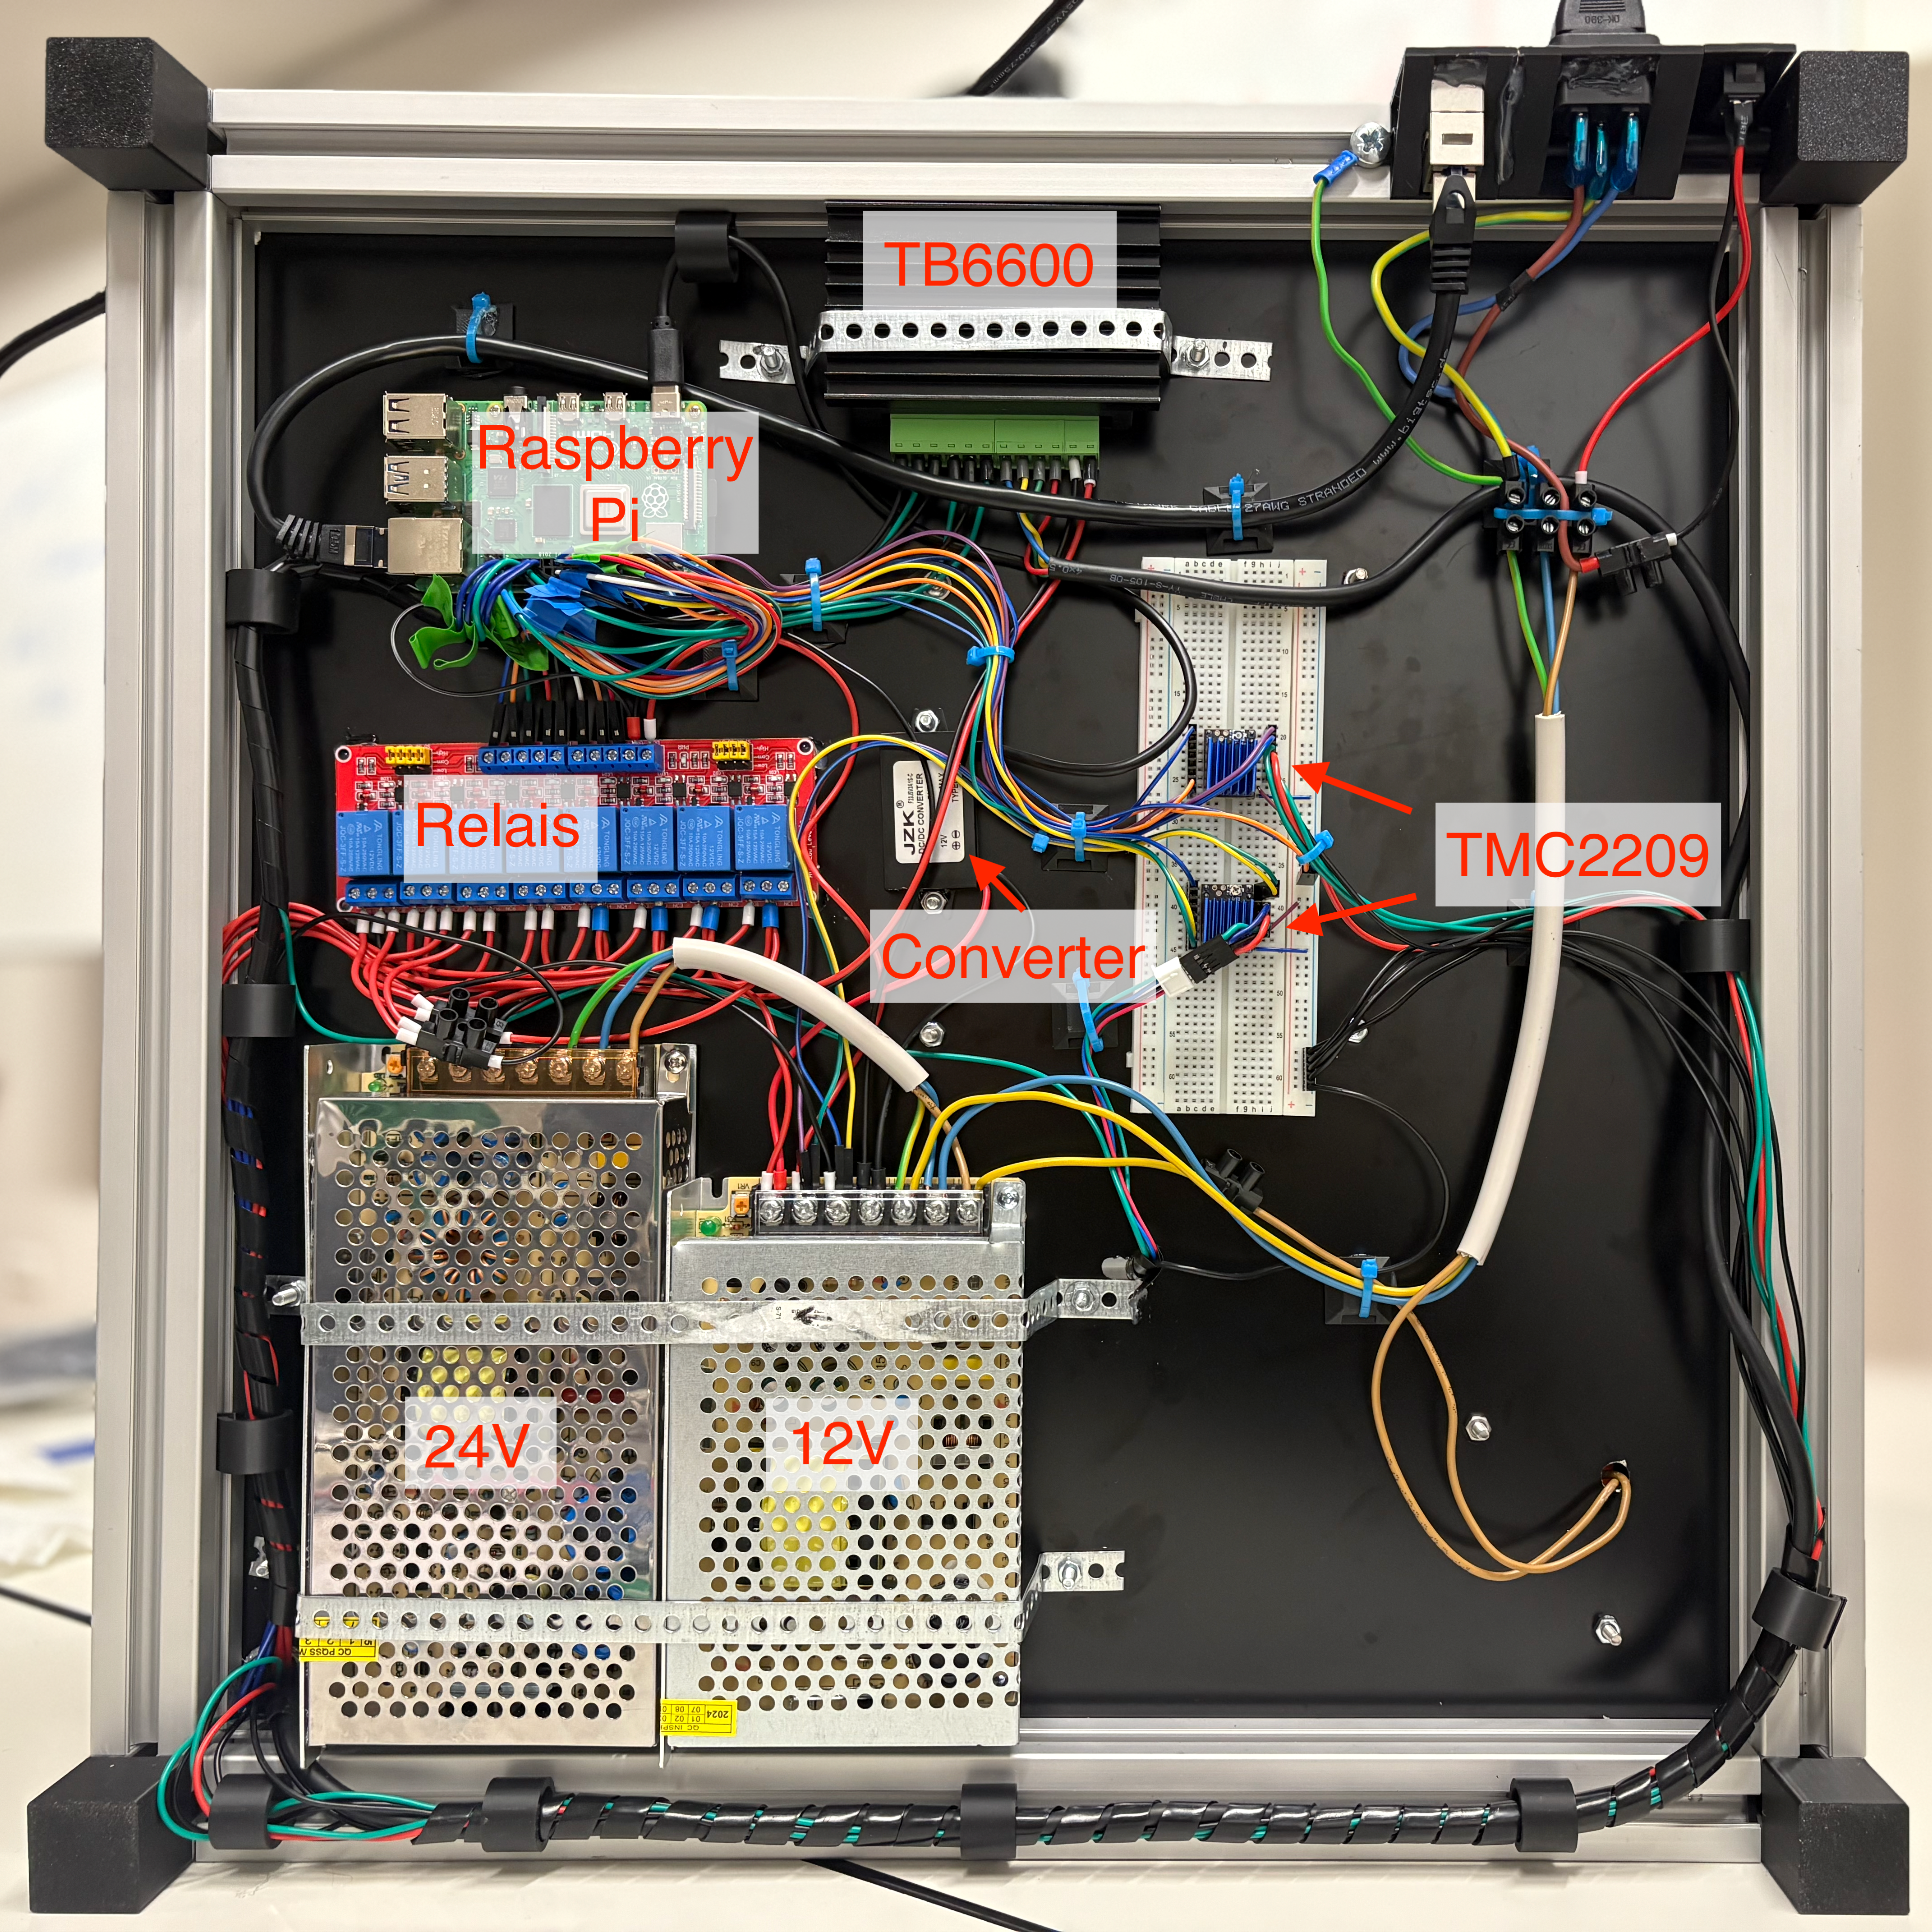
\includegraphics[width=0.8\textwidth]{images/unten.png}
    \caption{Elektronik auf der Unterseite des Probenverdünners}
    \label{fig:unten}
\end{figure}

Deswegen sollte dieser vorsichtig auf einem stabilen, und noch wichtiger, trockenem Untergrund platziert werden. Es sollte außerdem zu jeder Zeit darauf geachtet werden, dass keine Flüssigkeiten verschüttet werden; sowohl über, als auch neben dem Gerät, da dieses, zusätzlich zu der offenen Elektronik, auch Löcher für die Kabel einiger Geräte im Boden hat.\newpage

Sollte es dazu kommen, dass der Probenverdünner im laufenden Betrieb auf einen unerwarteten Fehler stößt oder beschädigt wird, ist sofort der Not-Aus-Schalter zu tätigen, siehe \autoref{fig:notaus}. 

\begin{figure}[H] % r = rechts, l = links
    \centering
    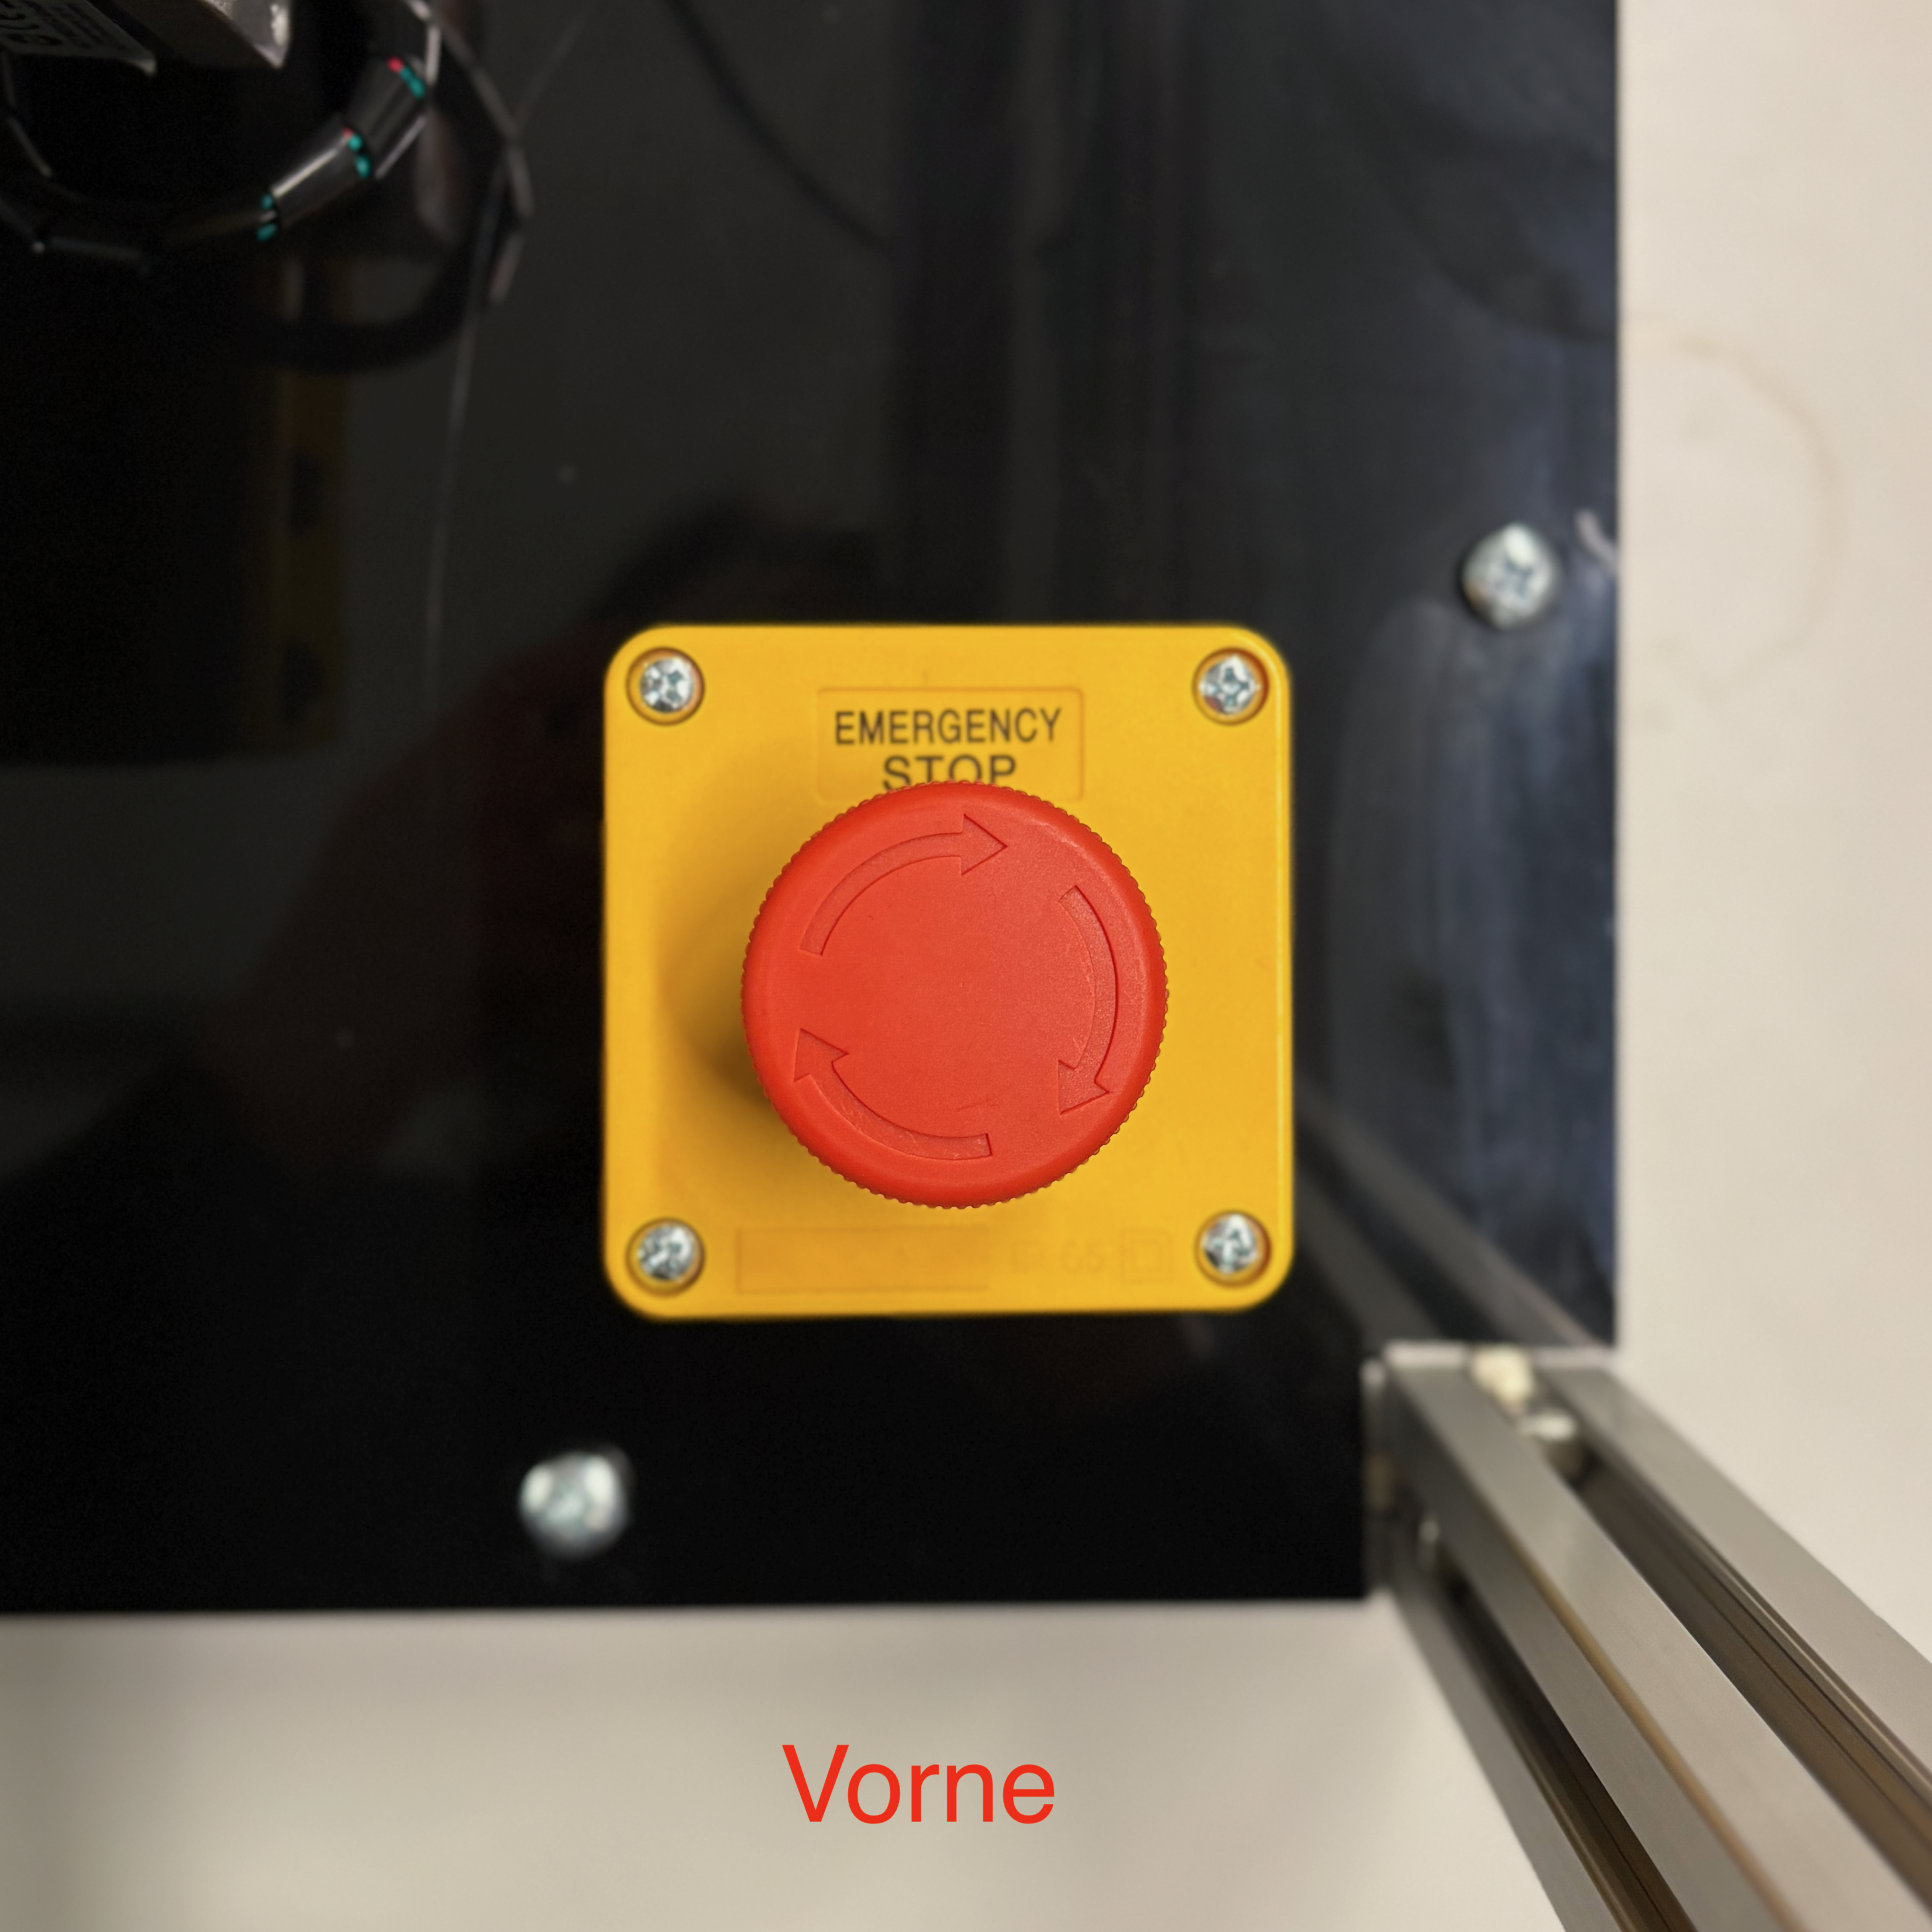
\includegraphics[width=0.45\textwidth]{images/notaus.png}
    \caption{Not-Aus des Probenverdünners}
    \label{fig:notaus}
\end{figure}

Nachdem dieser gedrückt wurde fährt sich sämtliche Elektronik des Geräts runter und alles bleibt dort stehen wo es ist. Um das Gerät nach dem Notfall wieder einzuschalten, muss der Not-Aus-Knopf einmal nach rechts gedreht werden.\\

Danach fährt das Gerät wieder hoch und der Zugriff auf die grafische Oberfläche ist möglich. Dort findet man den Button \textbf{Reset}, durch welchen der Probenverdünner zurück an die Nullpositionen fährt und alles resetet. Erst danach kann das Gerät wieder normal genutzt werden, siehe \autoref{fig:start}.\\

\begin{figure}[H] % r = rechts, l = links
    \centering
    \includegraphics[width=0.8\textwidth]{images/Startseite.png}
    \caption{GUI Startseite Reset Button}
    \label{fig:start}
\end{figure}

\subsection{Mechanische Sicherheitshinweise}\label{MechanischeSicherheitshinweise}
Aus Kostengründen wurden die Füße sowie die Steckerhalter für Netzwerk und Strom 3D-gedruckt. Diese sind zwar stabil aber können bei unvorsichtiger Benutzung brechen. Sollte dies auftreten, können die nötigen Pläne, um diese erneut zu drucken, im GitHub unter dem Ordner \textit{3D-Drucke} gefunden werden. \\

Es empfielt sich das Gerät nicht zu nutzen, solange die Teile noch nicht wieder ausgetauscht wurden. \\

Leider ist der gewählte Motor, welcher den Hubtisch antreibt, nicht stark genug, um die Last der Proben zusammen mit den Widerständen, die durch das Gewinde und die Führstangen des Hubtisches entstehen, zu bewegen. Daher wurde ein Expandierseil mit Haken zur Unterstützung an dem Rahmen und dem Hubtisch befestigt.\\

Während des gesamten Durchlaufs darf nichts in dem Pinkler landen. Insbesondere der Hubtisch und die Linearführung des Spritzkopfes stellen eine Quetschgefahr dar. Deshalb sollten lange Haare, Kleidung oder Schmuckstücke von den beweglichen Teilen ferngehalten werden, um ein Verfangen zu vermeiden. \

Zudem ist der Probenverdünner nicht für hohe Lasten geeignet. Das Gerät sollte somit nicht als Ablage oder Stütze genutzt werden.


